\documentclass{standalone}
\usepackage{pgfplots}
\pgfplotsset{compat=newest}
\begin{document}
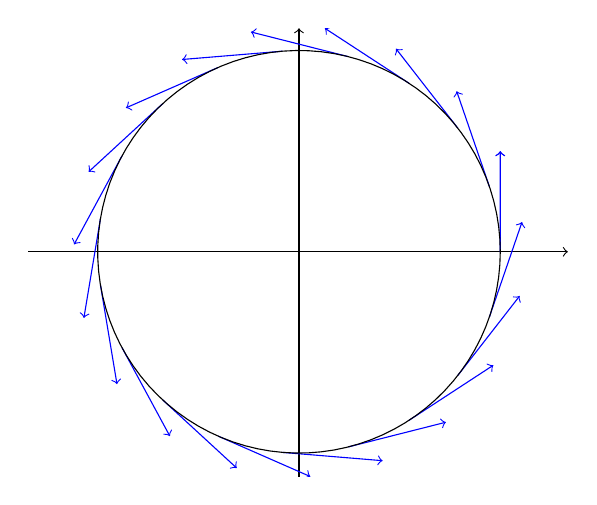
\begin{tikzpicture}
\begin{axis}[axis equal,
 axis lines=middle,
 axis line style={->},
 tick style={color=black},
 xtick=\empty,
 ytick=\empty
]
  \addplot[samples=20, domain=0:2*pi, 
	% the default choice 'variable=\x' leads to 
	% unexpected results here!
	variable=\t,
	quiver={
		u={-sin(deg(t))},
		v={cos(deg(t))},
		scale arrows=0.5},
		->,blue]
	({cos(deg(t))}, {sin(deg(t))});
  \addplot[samples=100, domain=0:2*pi] 
	({cos(deg(x))}, {sin(deg(x))});
\end{axis}
\end{tikzpicture}
\end{document}
